\clearpage
\subsection{MSVC + \olly}
\index{\olly}

\RU{Попробуем этот же пример в}\EN{Let's try this example in} \olly.
\RU{Загружаем, нажимаем F8 (\stepover) до тех пор, пока не окажемся в своем исполняемом файле,
а не в}\EN{Let's load it and keep pressing F8 (\stepover) until we reach our executable file
instead of} \TT{ntdll.dll}.
\RU{Скроллим вверх, до тех пока не найдем \main}\EN{Scroll up until \main appears}.
\RU{Кликаем на первой инструкции}\EN{Click on the first instruction} (\TT{PUSH EBP}), 
\RU{нажимаем}\EN{press} F2 (set a breakpoint), \RU{затем}\EN{then} F9 (Run) \RU{и брякпойнт срабатывает
на начале \main}\EN{. The breakpoint will be triggered when \main begins}.

\RU{Трассируем до того места, где готовится адрес переменной $x$}
\EN{Let's trace to the point where the address of the variable $x$ is calculated}:

\begin{figure}[H]
\centering
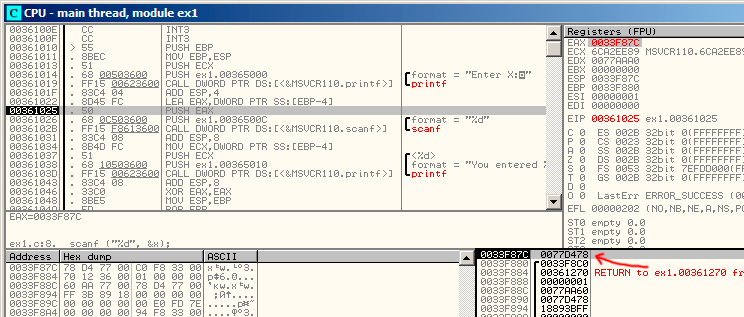
\includegraphics[scale=\FigScale]{patterns/04_scanf/1_simple/ex1_olly_1.png}
\caption{\olly: \RU{вычисляется адрес локальной переменной}\EN{The address of the local variable is calculated}}
\label{fig:scanf_ex1_olly_1}
\end{figure}

\RU{На \EAX в окне регистров можно нажать правой кнопкой и далее}
\EN{Right-click the \EAX in the registers window and then select} ``Follow in stack''.
\RU{Этот адрес покажется в окне стека}\EN{This address will appear in the stack window}.
\RU{Смотрите, это переменная в локальном стеке. Я нарисовал там красную стрелку}\EN{The red arrow, I have added, points to the variable in the local stack}.
\RU{И там сейчас какой-то мусор}\EN{At that moment this location contains some garbage} (\TT{0x6E494714}).
\RU{Адрес этого элемента стека сейчас, при помощи \PUSH, запишется в этот же стек, рядом}
\EN{Now with the help of \PUSH instruction the address of this stack element is going to be stored to the same stack on the next position}.
\RU{Трассируем при помощи F8 вплоть до конца исполнения \scanf}\EN{Let's trace with F8 until the \scanf execution completes}.
\RU{А пока \scanf исполняется, в консольном окне, вводим, например, 123}
\EN{During the \scanf execution, we input, for example, 123, in the console window}:

\begin{figure}[H]
\centering
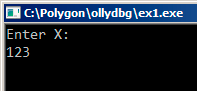
\includegraphics[scale=\NormalScale]{patterns/04_scanf/1_simple/ex1_olly_2.png}
\caption{\RU{Вывод в консоль}\EN{User input in the console window}}
\label{fig:scanf_ex1_olly_2}
\end{figure}

\clearpage
\RU{Вот тут }\scanf \RU{отработал}\EN{completed its execution already}:

\begin{figure}[H]
\centering
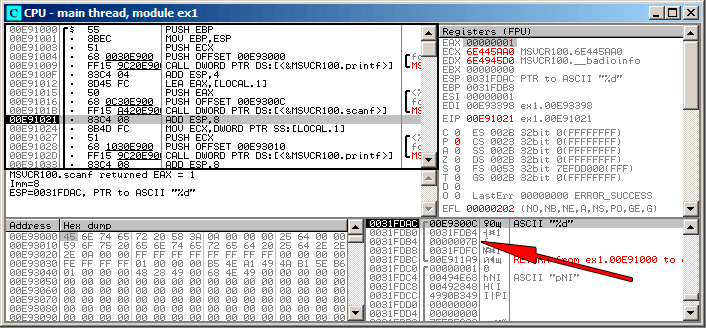
\includegraphics[scale=\FigScale]{patterns/04_scanf/1_simple/ex1_olly_3.png}
\caption{\olly: \scanf \RU{исполнилась}\EN{executed}}
\label{fig:scanf_ex1_olly_3}
\end{figure}

\scanf \RU{вернул}\EN{returns} $1$ \InENRU \EAX, \RU{что означает, что он успешно прочитал одно 
значение}\EN{which means that it has read successfully one value}.
\RU{В наблюдаемом нами элементе стека теперь}\EN{If we look again at the stack element corresponding to the local variable it now contains} \TT{0x7B} (123).

\clearpage
\RU{Чуть позже, это значение копируется из стека в регистр \ECX и передается в \printf}
\EN{Further, this value is copied from the stack to the \ECX register and passed to \printf}:

\begin{figure}[H]
\centering
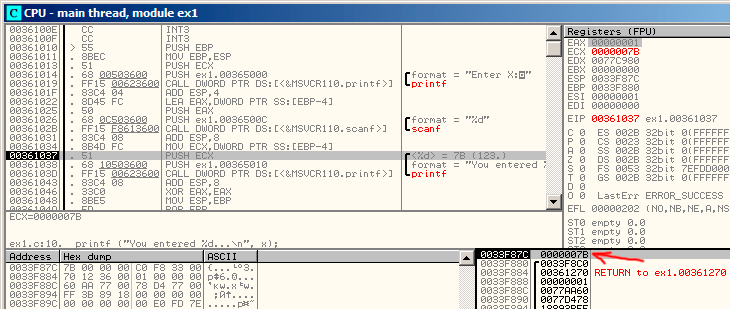
\includegraphics[scale=\FigScale]{patterns/04_scanf/1_simple/ex1_olly_4.png}
\caption{\olly: \RU{готовим значение для передачи в}\EN{preparing the value for passing to} \printf}
\label{fig:scanf_ex1_olly_4}
\end{figure}
